\documentclass[12pt,a4paper]{article}

\usepackage[T1]{fontenc}
\usepackage[utf8]{inputenc}
\usepackage[slovak]{babel}
\usepackage{geometry}
\usepackage{graphicx}
\usepackage{float}
\usepackage{booktabs}
\usepackage{tabularx}
\usepackage{hyperref}

\geometry{margin=2.5cm}
\graphicspath{{../schemy/}}

\title{Riadenie prevádzky veternej elektrárne\\Princípy informačných systémov}
\author{Kačmárová Lucia \and meno1 \and meno2}
\date{Akademický rok 2025/2026}

\begin{document}

\hypersetup{pageanchor=false}
\begin{titlepage}
  \centering
  {\Large Slovenská technická univerzita v Bratislave\par}
  {\Large Fakulta informatiky a informačných technológií\par}
  \vspace{3cm}
  {\huge\bfseries Riadenie prevádzky veternej elektrárne\par}
  \vspace{0.5cm}
  {\Large Princípy informačných systémov\par}
  \vspace{2.5cm}

  {\large Kačmárová Lucia, meno1, meno2\par}
  \vfill

  \begin{tabular}{rl}
    Cvičenie: & Štvrtok, 9:00 \\
    Cvičiaci: & Ádám Kemény \\
    Akademický rok: & 2025/2026 \\
  \end{tabular}
\end{titlepage}
\hypersetup{pageanchor=true}

\tableofcontents
\newpage

\section{Rámcová téma}
Téma projektu je zameraná na riadenie prevádzky veternej elektrárne, konkrétne na procesy spojené so spustením výroby elektriny, jej monitorovaním a riešením porúch. Veterná elektráreň je komplexný systém, ktorý zahŕňa automatizované riadiace prvky aj ľudské zásahy. Cieľom je zabezpečiť bezpečnú a stabilnú výrobu elektrickej energie v závislosti od aktuálnych podmienok.

V rámci tejto témy boli identifikované tri hlavné procesy:
\begin{enumerate}
  \item Spustenie výroby elektriny
  \item Monitorovanie a regulácia prevádzky
  \item Riešenie poruchy a obnovenie prevádzky
\end{enumerate}

\section{Proces 1 -- Spustenie výroby elektriny}
\subsection{Popis procesu}
Proces spustenia výroby elektriny začína získaním aktuálnych údajov o poveternostných podmienkach, predovšetkým o rýchlosti a smere vetra. Túto činnosť vykonáva riadiaci systém veternej elektrárne, ktorý priebežne zhromažďuje a vyhodnocuje meteorologické údaje. Následne riadiaci systém vykoná kontrolu technického stavu turbíny, pričom overuje funkčnosť základných komponentov, ako sú lopatky, generátor a brzdný systém.

Súčasťou prípravy je aj kontrola bezpečnostných limitov (napr. prekročenie maximálnej rýchlosti vetra, poruchové stavy a pod.). Po tejto kontrole sa realizuje kontrola pripojenia elektrárne do distribučnej siete, ktorú zabezpečuje dispečer distribučnej siete. Po vykonaní uvedených kontrol riadiaci systém vyhodnotí, či sú splnené prevádzkové podmienky na spustenie výroby elektriny. Ak podmienky nie sú splnené, proces sa ukončí. Ak sú podmienky vyhovujúce, riadiaci systém vykoná nastavenie turbíny (najmä natočenie gondoly a nastavenie prevádzkových parametrov) a následne spustí generátor. Po spustení generátora operátor elektrárne potvrdí úspešné spustenie výroby. Proces sa končí začiatkom výroby elektrickej energie a prechodom do procesu monitorovania a regulácie prevádzky.

\subsection{Procesné informácie (tokeny, prechody, stavy)}
\begin{table}[H]
  \centering
  \renewcommand{\arraystretch}{1.2}
  \begin{tabularx}{\textwidth}{|p{0.22\textwidth}|X|}
    \hline
    \textbf{Názov procesu} & Spustenie výroby elektriny \\
    \hline
    \textbf{Popis} & Na základe údajov o vetre a kontrol technického stavu systém rozhodne o spustení výroby. Prebehne paralelná kontrola bezpečnostných limitov a pripojenia do distribučnej siete. Ak sú podmienky splnené, turbína sa nastaví, spustí sa generátor a operátor potvrdí spustenie. \\
    \hline
    \textbf{Roly} & Riadiaci systém (RS), Operátor elektrárne (O), Dispečer distribučnej siete (DDS) \\
    \hline
    \textbf{Vstupné tokeny} & Aktuálne meteorologické údaje (rýchlosť/smer vetra), technický stav turbíny, informácia o dostupnosti pripojenia do siete \\
    \hline
    \textbf{Výstupné tokeny} & Stav \emph{Výroba spustená} alebo \emph{Proces ukončený} (podmienky nesplnené) \\
    \hline
    \textbf{Prechody} & Získaj údaje o vetre, skontroluj technický stav, skontroluj bezpečnostné limity, over pripojenie do siete, vyhodnoť podmienky, nastav turbínu, spusť generátor, potvrď spustenie výroby \\
    \hline
    \textbf{Stavy} & Údaje o vetre získané, technický stav overený, bezpečnostné limity overené, pripojenie do siete overené, podmienky vyhodnotené, turbína nastavená, generátor spustený, výroba spustená \\
    \hline
  \end{tabularx}
  \caption{Proces 1 -- Zhrnutie procesu}
\end{table}

\subsection{Procesné roly}
\begin{table}[H]
  \centering
  \renewcommand{\arraystretch}{1.2}
  \begin{tabularx}{\textwidth}{|p{0.22\textwidth}|X|}
    \hline
    \textbf{Rola} & \textbf{Úloha} \\
    \hline
    Riadiaci systém & Zbiera a vyhodnocuje meteorologické údaje, kontroluje technický stav a bezpečnostné limity, rozhoduje o spustení, vykonáva nastavenie turbíny a spúšťa generátor. \\
    \hline
    Operátor elektrárne & Vykoná finálne potvrdenie spustenia výroby a môže zasiahnuť pri neštandardných situáciách (napr. manuálne potvrdenie alebo zrušenie spustenia). \\
    \hline
    Dispečer distribučnej siete & Overuje a potvrdzuje pripojenie do distribučnej siete (možnosť dodávky/odberu) pred spustením výroby. \\
    \hline
  \end{tabularx}
  \caption{Proces 1 -- Popis rolí}
\end{table}

\subsection{Procesné roly (priradenie činností)}
\begin{table}[H]
  \centering
  \small
  \renewcommand{\arraystretch}{1.2}
  \begin{tabularx}{\textwidth}{|X|p{0.17\textwidth}|p{0.17\textwidth}|p{0.17\textwidth}|}
    \hline
    \textbf{Činnosť} & \textbf{RS} & \textbf{O} & \textbf{DDS} \\
    \hline
    Získaj údaje o vetre & X &  &  \\
    \hline
    Skontroluj technický stav turbíny & X &  &  \\
    \hline
    Skontroluj bezpečnostné limity & X &  &  \\
    \hline
    Over pripojenie do siete &  &  & X \\
    \hline
    Vyhodnoť prevádzkové podmienky & X &  &  \\
    \hline
    Nastav turbínu & X &  &  \\
    \hline
    Spusť generátor & X &  &  \\
    \hline
    Potvrď spustenie výroby &  & X &  \\
    \hline
  \end{tabularx}
  \caption{Proces 1 -- Priradenie činností k rolám}
\end{table}

\subsection{Petriho sieť}
Model procesu bol navrhnutý ako Petriho sieť v nástroji Netgrif Builder. Model obsahuje rozhodovanie (XOR split), paralelné vetvenie (AND split), dátové polia (enumeration) a TaskRef na úlohu z iného procesu.
\begin{figure}[H]
  \centering
  
\includegraphics[width=\textwidth]{petri/proces1-spustenie.png}
  \caption{Proces 1 -- Petriho sieť}
\end{figure}

\subsection{Graf dosiahnuteľnosti}
\emph{TODO: Sem doplniť graf dosiahnuteľnosti pre vybraný proces.}

\subsection{Obrazovky}
\emph{TODO: Sem doplniť návrh obrazoviek pre prechody Petriho siete.}

\subsection{BPMN}
\begin{figure}[H]
  \centering
  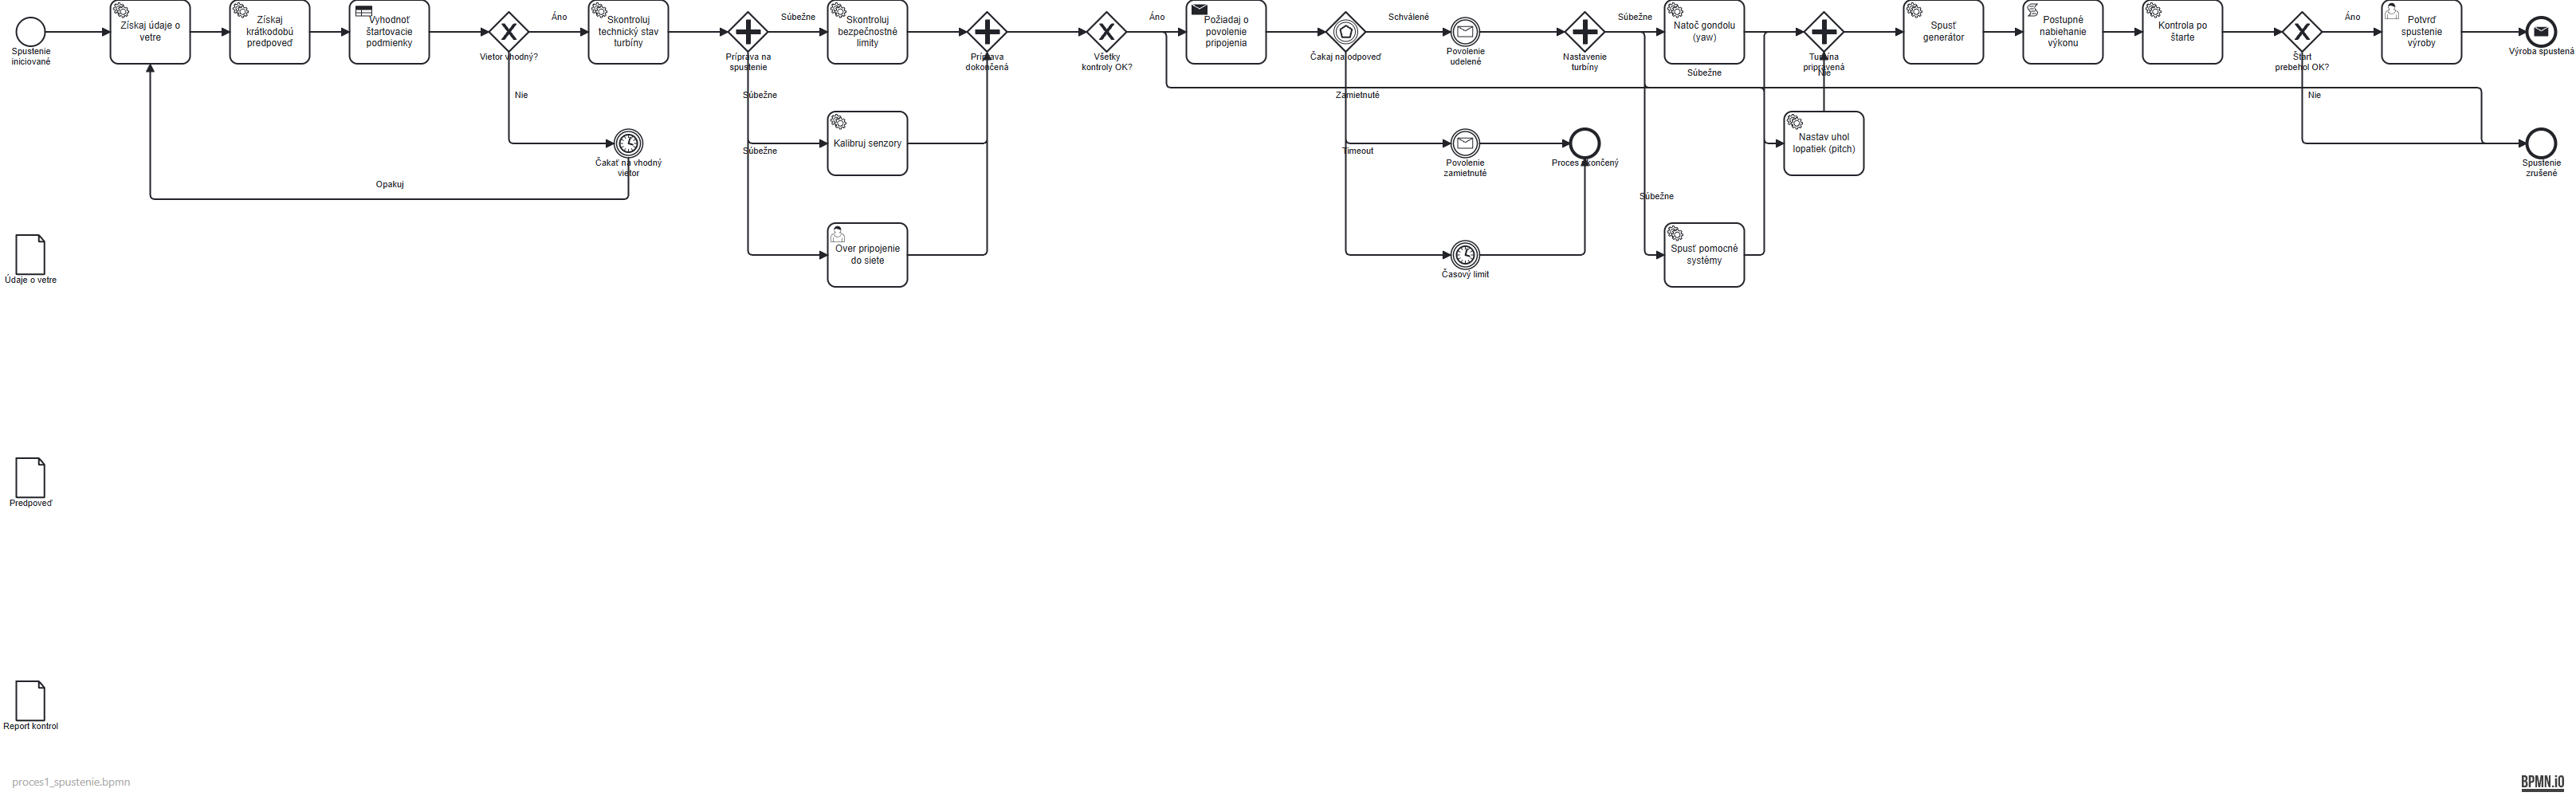
\includegraphics[width=\textwidth]{bpmn/proces1-spustenie.png}
  \caption{Proces 1 -- BPMN model}
\end{figure}

\section{Proces 2 -- Monitorovanie a regulácia prevádzky}
\subsection{Popis procesu}
Proces monitorovania a regulácie prevádzky začína po úspešnom spustení výroby elektriny. Riadiaci systém nepretržite sleduje základné prevádzkové parametre veternej elektrárne, ako sú rýchlosť vetra, výkon generátora a ďalšie technické ukazovatele. Následne dochádza k vyhodnoteniu získaných údajov s cieľom určiť, či prevádzka elektrárne prebieha stabilne.

Vyhodnocovanie údajov prebieha periodicky (v pravidelných intervaloch) alebo okamžite pri detekcii alarmu/odchýlky. Ak je prevádzka stabilná, riadiaci systém vykoná optimalizáciu výkonu a následne sa odosielajú údaje o výrobe elektriny dispečerovi distribučnej siete. Po odoslaní údajov sa proces opakuje a opätovne pokračuje sledovaním parametrov. Ak prevádzka nie je stabilná, vyhodnocuje sa závažnosť odchýlky. V prípade menej závažnej odchýlky vykoná operátor elektrárne úpravu prevádzkových parametrov a proces sa následne vracia späť do fázy monitorovania. Ak ide o závažnú odchýlku alebo poruchu, proces monitorovania sa ukončí a nadväzuje na proces riešenia poruchy a obnovenia prevádzky.

\subsection{Procesné informácie (tokeny, prechody, stavy)}
\begin{table}[H]
  \centering
  \renewcommand{\arraystretch}{1.2}
  \begin{tabularx}{\textwidth}{|p{0.22\textwidth}|X|}
    \hline
    \textbf{Názov procesu} & Monitorovanie a regulácia prevádzky \\
    \hline
    \textbf{Popis} & Systém zbiera a predspracuje senzorové dáta, paralelne sleduje vietor/výkon a technické indikátory a v intervaloch alebo pri alarme vyhodnocuje stabilitu. Pri stabilnej prevádzke vypočíta optimálne nastavenia, paralelne upraví pitch/yaw/menič, overí bezpečnostné limity a odošle údaje o výrobe dispečerovi. Ak limity nie sú splnené alebo ide o menšiu odchýlku, vyžiada zásah operátora (fyzická kontrola, úprava parametrov). Pri závažnej odchýlke prejde na riešenie poruchy. Dispečer môže poslať požiadavku na reguláciu výkonu, ktorú operátor potvrdí a systém upraví setpoint. \\
    \hline
    \textbf{Roly} & Riadiaci systém (RS), Operátor elektrárne (O), Dispečer distribučnej siete (DDS) \\
    \hline
    \textbf{Vstupné tokeny} & Priebežné merania (rýchlosť vetra, výkon, teploty, vibrácie), alarm/odchýlka zo senzorov, požiadavka na reguláciu výkonu (DDS) \\
    \hline
    \textbf{Výstupné tokeny} & Odoslané a zaevidované údaje o výrobe, potvrdená regulácia výkonu, upravené prevádzkové parametre alebo stav \emph{Prechod na riešenie poruchy} \\
    \hline
    \textbf{Prechody} & Zbieraj senzorové dáta, predspracuj dáta, paralelné monitorovanie (vietor/výkon, teploty/vibrácie), čakaj na udalosť (čas/alarm/DDS), vyhodnoť údaje, vypočítaj optimálne nastavenia, nastav pitch/yaw/menič, over limity, odošli údaje o výrobe, zaeviduj údaje v sieti, klasifikuj odchýlku, vyžiadaj zásah operátora, fyzická kontrola, úprava parametrov, úprava setpointu, potvrdenie regulácie, prechod na riešenie poruchy \\
    \hline
    \textbf{Stavy} & Dáta zozbierané, dáta predspracované, monitorovanie vykonané, udalosť zachytená, stabilita vyhodnotená, nastavenia aplikované, limity OK/NOK, údaje odoslané a zaevidované, odchýlka klasifikovaná, operátor informovaný, parametre upravené, setpoint upravený, regulácia zaevidovaná, prechod na poruchu \\
    \hline
  \end{tabularx}
  \caption{Proces 2 -- Zhrnutie procesu}
\end{table}

\subsection{Procesné roly}
\begin{table}[H]
  \centering
  \renewcommand{\arraystretch}{1.2}
  \begin{tabularx}{\textwidth}{|p{0.22\textwidth}|X|}
    \hline
    \textbf{Rola} & \textbf{Úloha} \\
    \hline
    Riadiaci systém & Zbiera a predspracúva senzorové dáta, spracúva alarmy, vyhodnocuje stabilitu prevádzky, počíta a aplikuje optimálne nastavenia (pitch/yaw/menič), overuje limity, odosiela údaje dispečerovi a vykonáva zmeny parametrov/setpointu. \\
    \hline
    Operátor elektrárne & Preskúmava odchýlky, podľa potreby vykonáva fyzickú kontrolu a upravuje prevádzkové parametre; potvrdzuje požiadavky DDS na reguláciu výkonu. \\
    \hline
    Dispečer distribučnej siete & Eviduje údaje o výrobe a regulácie v sieti a môže poslať požiadavku na reguláciu výkonu (podľa situácie v sieti). \\
    \hline
  \end{tabularx}
  \caption{Proces 2 -- Popis rolí}
\end{table}

\subsection{Procesné roly (priradenie činností)}
\begin{table}[H]
  \centering
  \small
  \renewcommand{\arraystretch}{1.2}
  \begin{tabularx}{\textwidth}{|X|p{0.17\textwidth}|p{0.17\textwidth}|p{0.17\textwidth}|}
    \hline
    \textbf{Činnosť} & \textbf{RS} & \textbf{O} & \textbf{DDS} \\
    \hline
    Zbieraj senzorové dáta & X &  &  \\
    \hline
    Predspracuj dáta (filtrácia) & X &  &  \\
    \hline
    Sleduj vietor a výkon & X &  &  \\
    \hline
    Sleduj teploty a vibrácie & X &  &  \\
    \hline
    Čakaj na udalosť (čas/alarm/DDS) & X &  &  \\
    \hline
    Vyhodnoť údaje & X &  &  \\
    \hline
    Vypočítaj optimálne nastavenia & X &  &  \\
    \hline
    Nastav uhol lopatiek (pitch) & X &  &  \\
    \hline
    Natoč gondolu (yaw) & X &  &  \\
    \hline
    Nastav menič/brzdy & X &  &  \\
    \hline
    Over bezpečnostné limity & X &  &  \\
    \hline
    Odošli údaje o výrobe & X &  &  \\
    \hline
    Zaeviduj údaje v sieti &  &  & X \\
    \hline
    Klasifikuj odchýlku & X &  &  \\
    \hline
    Vyžiadaj zásah operátora & X &  &  \\
    \hline
    Preskúmaj odchýlku &  & X &  \\
    \hline
    Fyzická kontrola turbíny &  & X &  \\
    \hline
    Uprav prevádzkové parametre &  & X &  \\
    \hline
    Aplikuj zmeny v systéme & X &  &  \\
    \hline
    Zaznamenaj zmeny & X &  &  \\
    \hline
    Potvrď požiadavku DDS &  & X &  \\
    \hline
    Uprav setpoint výkonu & X &  &  \\
    \hline
    Odošli potvrdenie DDS & X &  &  \\
    \hline
    Zaeviduj reguláciu v sieti &  &  & X \\
    \hline
    Prechod na riešenie poruchy & X &  &  \\
    \hline
  \end{tabularx}
  \caption{Proces 2 -- Priradenie činností k rolám}
\end{table}

\subsection{Petriho sieť}
Model procesu bol navrhnutý ako Petriho sieť v nástroji Netgrif Builder. Model obsahuje rozhodovanie (XOR split), paralelné vetvenie (AND split), dátové polia (multichoice\_map) a TaskRef na úlohu z iného procesu.
\begin{figure}[H]
  \centering
  
\includegraphics[width=\textwidth]{petri/proces2-monitorovanie.png}
  \caption{Proces 2 -- Petriho sieť}
\end{figure}

\subsection{Graf dosiahnuteľnosti}
\emph{TODO: Sem doplniť graf dosiahnuteľnosti pre vybraný proces.}

\subsection{Obrazovky}
\emph{TODO: Sem doplniť návrh obrazoviek pre prechody Petriho siete.}

\subsection{BPMN}
\begin{figure}[H]
  \centering
  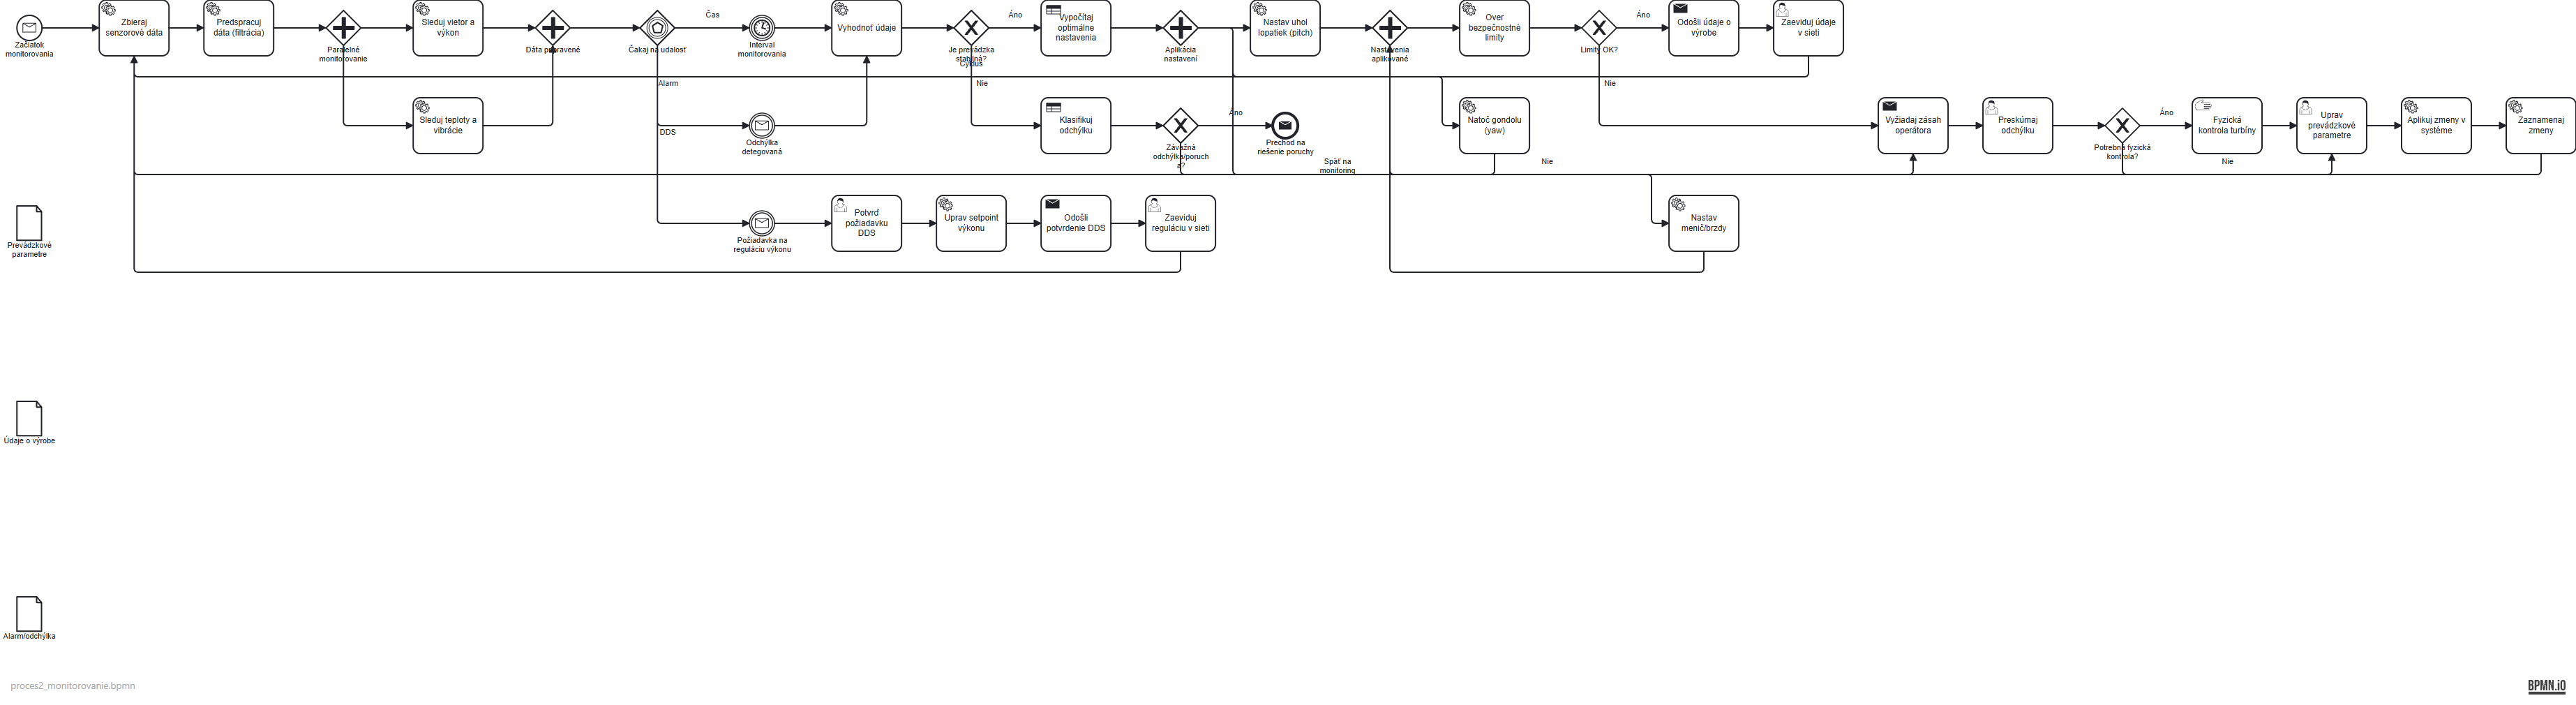
\includegraphics[width=\textwidth]{bpmn/proces2-monitorovanie.png}
  \caption{Proces 2 -- BPMN model}
\end{figure}

\section{Proces 3 -- Riešenie poruchy a obnovenie prevádzky}
\subsection{Popis procesu}
Proces riešenia poruchy začína zaznamenaním poruchového hlásenia. Poruchu najskôr deteguje riadiaci systém, ktorý zároveň zaznamená hlásenie o vzniknutej poruche. Následne operátor elektrárne vyhodnotí situáciu a rozhoduje, či ide o kritickú poruchu. Ak ide o kritickú poruchu, riadiaci systém vykoná núdzové zastavenie turbíny. Ak porucha nie je kritická, operátor zabezpečí plánované odstavenie zariadenia.

Po odstavení zariadenia sa riadiacim systémom vytvorí servisná úloha, na základe ktorej servisný technik vykoná diagnostiku problému a následne realizuje opravu. Po dokončení opravy servisný technik vykoná test funkčnosti zariadenia. Na základe výsledku testu sa rozhodne, či je zariadenie v poriadku. Ak je zariadenie funkčné, riadiaci systém zabezpečí opätovné spustenie výroby a dispečer distribučnej siete je informovaný o obnovení dodávky. Proces sa tým končí obnovením prevádzky. Ak zariadenie nie je v poriadku, problém sa eskaluje a proces riešenia sa opakuje až do úspešného odstránenia poruchy alebo odovzdania problému na vyššiu úroveň riešenia.
Ak oprava trvá neprimerane dlho, operátor elektrárne eskaluje problém (napr. na vyššiu úroveň podpory).

\subsection{Procesné informácie (tokeny, prechody, stavy)}
\begin{table}[H]
  \centering
  \renewcommand{\arraystretch}{1.2}
  \begin{tabularx}{\textwidth}{|p{0.22\textwidth}|X|}
    \hline
    \textbf{Názov procesu} & Riešenie poruchy a obnovenie prevádzky \\
    \hline
    \textbf{Popis} & Po detekcii poruchy systém zaznamená hlásenie, zhromaždí diagnostické údaje a operátor rozhodne o kritickosti. Pri kritickej poruche prebehne núdzové zastavenie, inak plánované odstavenie. Po odstavení sa paralelne vytvorí servisná úloha, informuje sa dispečer a zabezpečí sa prístup a bezpečnosť na mieste. Servisný technik vykoná diagnostiku a opravu; ak je potrebný náhradný diel, čaká sa na dodávku a rieši sa oneskorenie. Po úspešnej oprave systém požiada DDS o opätovné pripojenie (schválenie/zamietnutie/timeout) a po schválení obnoví výrobu a odošle oznámenie, ktoré DDS zaeviduje. Pri dlhom riešení môže operátor incident eskalovať. \\
    \hline
    \textbf{Roly} & Riadiaci systém (RS), Operátor elektrárne (O), Servisný technik (ST), Dispečer distribučnej siete (DDS) \\
    \hline
    \textbf{Vstupné tokeny} & Poruchové hlásenie (alarm), diagnostické údaje, servisná požiadavka, dostupnosť pripojenia do siete (DDS), náhradné diely \\
    \hline
    \textbf{Výstupné tokeny} & Prevádzka obnovená + zaevidovanie v DDS alebo eskalovaný incident / odložené pripojenie (opakovaná žiadosť) \\
    \hline
    \textbf{Prechody} & Deteguj poruchu, zaznamenaj hlásenie, zhromaždi diagnostické údaje, vyhodnoť situáciu, rozhodni kritickosť, núdzové zastavenie / plánované odstavenie, vytvor servisnú úlohu, informuj DDS o odstávke, zaeviduj odstávku, zabezpeč prístup, diagnostika na mieste, čakanie na diel / urgencia, výmena dielu, oprava/kalibrácia, test funkčnosti, rozhodni či je zariadenie OK, požiadaj o opätovné pripojenie, čakaj na odpoveď DDS, naplánuj opätovnú žiadosť / kontaktuj DDS, opätovne spusti výrobu, odošli oznámenie o obnovení, zaeviduj obnovu, eskaluj problém \\
    \hline
    \textbf{Stavy} & Porucha detegovaná, hlásenie zaznamenané, diagnostické údaje pripravené, turbína odstavená, servisná úloha vytvorená, DDS informovaná, odstávka zaevidovaná, prístup zabezpečený, diagnostika vykonaná, diel potrebný/nepotrebný, diel doručený/oneskorený, oprava vykonaná, test vykonaný, zariadenie OK/nie OK, žiadosť o pripojenie odoslaná, odpoveď DDS prijatá (schválené/zamietnuté/timeout), výroba obnovená, obnova zaevidovaná, incident eskalovaný \\
    \hline
  \end{tabularx}
  \caption{Proces 3 -- Zhrnutie procesu}
\end{table}

\subsection{Procesné roly}
\begin{table}[H]
  \centering
  \renewcommand{\arraystretch}{1.2}
  \begin{tabularx}{\textwidth}{|p{0.22\textwidth}|X|}
    \hline
    \textbf{Rola} & \textbf{Úloha} \\
    \hline
    Riadiaci systém & Deteguje poruchu, zaznamenáva hlásenia, zhromažďuje diagnostické údaje, vykonáva núdzové zastavenie (ak treba), vytvára servisnú úlohu, informuje DDS, žiada o opätovné pripojenie a po schválení zabezpečuje obnovenie výroby a odoslanie oznámenia. \\
    \hline
    Operátor elektrárne & Vyhodnocuje situáciu, rozhoduje o kritickosti poruchy a o type odstavenia; zabezpečuje prístup a bezpečnosť, pri zamietnutí/timeoutoch koordinuje opakovanú žiadosť a pri dlhom riešení eskaluje incident. \\
    \hline
    Servisný technik & Vykonáva diagnostiku na mieste, realizuje opravu/kalibráciu a test funkčnosti; ak je potrebný náhradný diel, rieši čakanie a výmenu dielu, následne rozhoduje o pripravenosti zariadenia na spustenie. \\
    \hline
    Dispečer distribučnej siete & Eviduje odstávku a obnovu dodávky v sieti a poskytuje odpoveď na žiadosť o opätovné pripojenie (schválenie/zamietnutie). \\
    \hline
  \end{tabularx}
  \caption{Proces 3 -- Popis rolí}
\end{table}

\subsection{Procesné roly (priradenie činností)}
\begin{table}[H]
  \centering
  \small
  \renewcommand{\arraystretch}{1.2}
  \begin{tabularx}{\textwidth}{|X|p{0.14\textwidth}|p{0.14\textwidth}|p{0.14\textwidth}|p{0.14\textwidth}|}
    \hline
    \textbf{Činnosť} & \textbf{RS} & \textbf{O} & \textbf{ST} & \textbf{DDS} \\
    \hline
    Deteguj poruchu & X &  &  &  \\
    \hline
    Zaznamenaj hlásenie & X &  &  &  \\
    \hline
    Zhromaždi diagnostické údaje & X &  &  &  \\
    \hline
    Vyhodnoť situáciu &  & X &  &  \\
    \hline
    Rozhodni kritickosť poruchy &  & X &  &  \\
    \hline
    Núdzové zastavenie turbíny & X &  &  &  \\
    \hline
    Plánované odstavenie &  & X &  &  \\
    \hline
    Vytvor servisnú úlohu & X &  &  &  \\
    \hline
    Informuj DDS o odstávke & X &  &  &  \\
    \hline
    Zaeviduj odstávku v sieti &  &  &  & X \\
    \hline
    Zabezpeč prístup a bezpečnosť &  & X &  &  \\
    \hline
    Diagnostika na mieste &  &  & X &  \\
    \hline
    Urgencia dodávky dielu &  &  & X &  \\
    \hline
    Vymeň náhradný diel &  &  & X &  \\
    \hline
    Oprava/kalibrácia &  &  & X &  \\
    \hline
    Test funkčnosti zariadenia &  &  & X &  \\
    \hline
    Rozhodni či je zariadenie OK &  &  & X &  \\
    \hline
    Požiadaj o opätovné pripojenie & X &  &  &  \\
    \hline
    Naplánuj opätovnú žiadosť &  & X &  &  \\
    \hline
    Kontaktuj DDS &  & X &  &  \\
    \hline
    Opätovne spusti výrobu & X &  &  &  \\
    \hline
    Odošli oznámenie o obnovení & X &  &  &  \\
    \hline
    Zaeviduj obnovu dodávky &  &  &  & X \\
    \hline
    Eskaluj problém &  & X &  &  \\
    \hline
  \end{tabularx}
  \caption{Proces 3 -- Priradenie činností k rolám}
\end{table}

\subsection{Petriho sieť}
Model procesu bol navrhnutý ako Petriho sieť v nástroji Netgrif Builder. Model obsahuje rozhodovanie (XOR split), paralelné vetvenie (AND split), dátové polia (enumeration\_map) a TaskRef na úlohu z iného procesu.
\begin{figure}[H]
  \centering
  
\includegraphics[width=\textwidth]{petri/proces3-porucha.png}
  \caption{Proces 3 -- Petriho sieť}
\end{figure}

\subsection{Graf dosiahnuteľnosti}
\emph{TODO: Sem doplniť graf dosiahnuteľnosti pre vybraný proces.}

\subsection{Obrazovky}
\emph{TODO: Sem doplniť návrh obrazoviek pre prechody Petriho siete.}

\subsection{BPMN}
\begin{figure}[H]
  \centering
  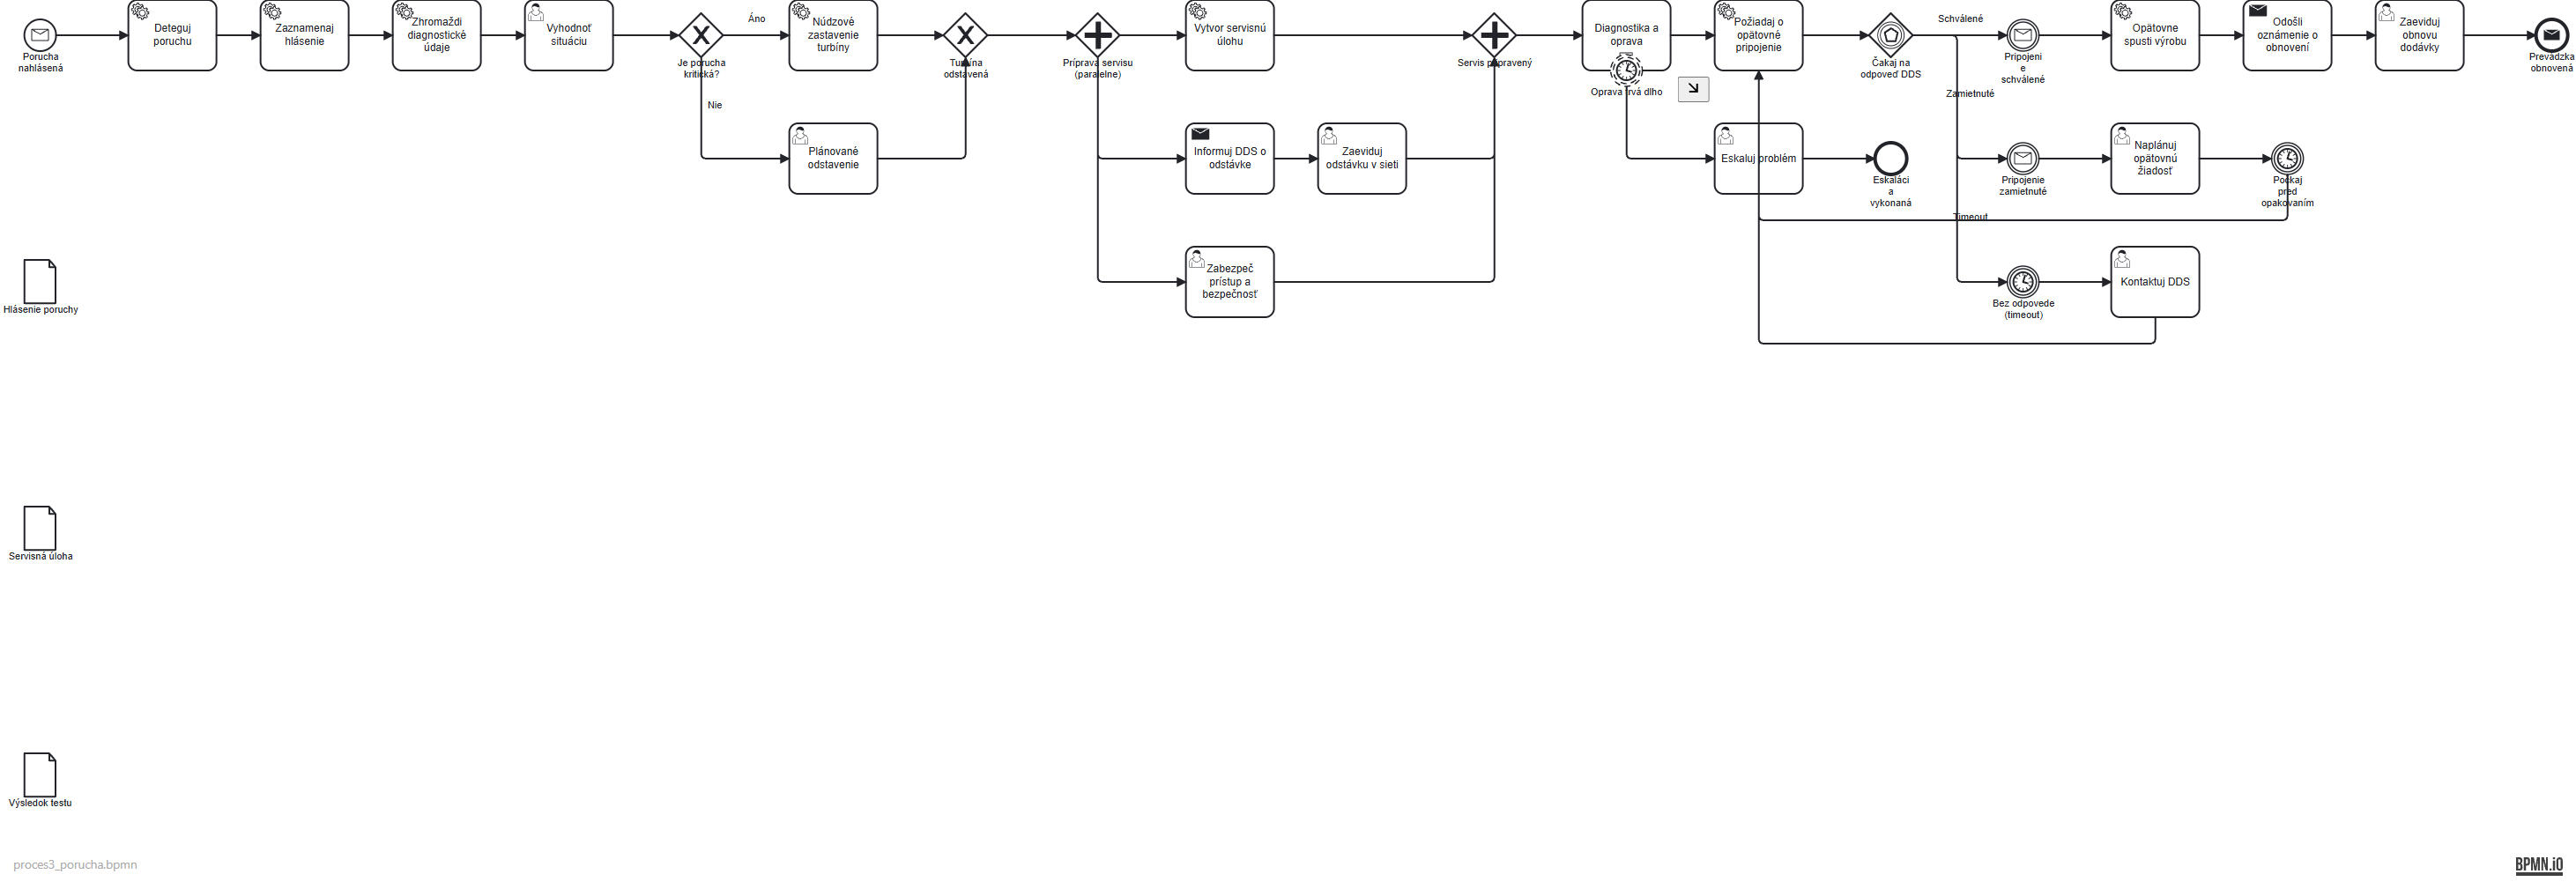
\includegraphics[width=\textwidth]{bpmn/proces3-porucha.png}
  \caption{Proces 3 -- BPMN model}
\end{figure}

\section{Poznámky k súladu so zadaním}
\begin{itemize}
  \item Slovné popisy: v dokumente sú popísané 3 procesy (splnené).
  \item Procesné roly: v dokumente sú tabuľky rolí a činností pri každom procese; celkovo sú identifikované minimálne 4 roly (splnené).
  \item BPMN: doplnené AND/XOR brány, event-based brána, cyklus, podproces, boundary event a artefakty (splnené).
  \item Petriho siete: doplnené obrázky modelov procesov (splnené).
  \item Grafy dosiahnuteľnosti a obrazovky: ponechané ako TODO (doplní sa v ďalšom kroku).
\end{itemize}

\end{document}
